
%----------------------------------------------------------------------------------------
%	PACKAGES AND OTHER DOCUMENT CONFIGURATIONS
%----------------------------------------------------------------------------------------

\documentclass{beamer}

\usetheme[hideothersubsections]{Goettingen}
\usepackage{algorithm}
\usepackage{algpseudocode}
\usepackage{graphicx}
\usepackage{subcaption}
\usepackage{amsmath}
\usepackage{amsthm}
\usepackage{caption}

% Declare theorem style and numbering
\theoremstyle{plain}
\newtheorem{thm}{Theorem}
\newtheorem{lem}{Lemma}
\newtheorem{corr}{Korrolar}
\theoremstyle{definition}
\newtheorem{defn}[thm]{Definition}
\newtheorem{ex}[thm]{Beispiel}

\newcommand{\mat}[1]{\mathbf{#1}}
\DeclareMathOperator*{\argmax}{arg\,max}
\DeclareMathOperator*{\argmin}{arg\,min}
\newcommand{\norm}[1]{\left\lVert #1 \right\rVert}

%----------------------------------------------------------------------------------------
%	BEGIN DOCUMENT
%----------------------------------------------------------------------------------------


\begin{document}

\title{Sparse Principal Component Analysis}
\subtitle{for Frequency Data}   
\institute{Institute for Numerical Simulation}
\author{Tobias Bork} 
\date{\today}
\titlegraphic{	\vspace{0.5cm}
				
\includegraphics[scale=0.04]{figures/university_of_bonn.png} 				\hspace{1cm}
				
\includegraphics[scale=0.10]{figures/fraunhofer_scai.png}}

\begin{frame}
\titlepage
\end{frame}

%\begin{frame}
%\frametitle{Table of Contents}
%\tableofcontents
%\end{frame}

%----------------------------------------------------------------------------------------
%	Introduction
%----------------------------------------------------------------------------------------

\section{Introduction} 
\begin{frame}
\frametitle{Dimensionality Reduction} 

\begin{itemize}
\item \textbf{Problems} in high dimensions: 
\setbeamertemplate{itemize items}[circle]
	\begin{itemize}
	\item Time and storage space
	\item Multi-collinearity 
	\item Visualizing data set
	\item Curse of dimensionality
	\end{itemize}
\setbeamertemplate{itemize items}[triangle]
\item \textbf{Idea:} Reduce the number of variables while preserving structure in the data
\item \textbf{Approach:} Feature selection methods
\item \textbf{Approach:} Feature extraction methods

\end{itemize}
\end{frame}

%----------------------------------------------------------------------------------------
%	Principal Component Analysis
%----------------------------------------------------------------------------------------

\section{PCA} 
\subsection{Idea}
\begin{frame}\frametitle{Central Idea}
\begin{itemize}
\item Reduce dimensionality while retaining as much information as possible
\item Sequentially identify principal axis of greatest variability
\item Represent data set regarding identified principal axis
\item Linearly project the data to a space of fewer dimensions
\item Yields natural order on principal components
\end{itemize} 
\end{frame}

\begin{frame}
\begin{figure}
\centering
	\begin{subfigure}{0.45\textwidth}
	\centering
	\captionsetup{justification=centering}
	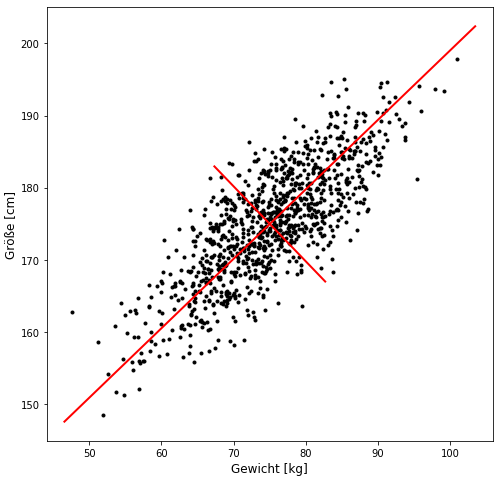
\includegraphics[width = \textwidth]{figures/pca_example.png}
	\label{pca_example_original}
	\caption{Finding principal axis on a data set}
	\end{subfigure}
	%	
	\begin{subfigure}{0.45\textwidth}
	\centering
	\captionsetup{justification=centering}
	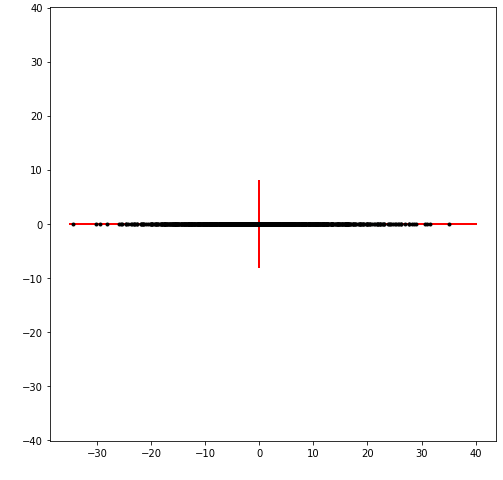
\includegraphics[width = \textwidth]{figures/pca_example_rotated.png}
	\label{pca_example_rotated}
	\caption{Linear projection of data to a space of fewer dimensions}
	\end{subfigure}

\label{pca_example}
\end{figure}
\end{frame}

\subsection{Mathematical Formulations}
\begin{frame}
\frametitle{Mathematical Formulation}
Let $\mat X \in \mathbb{R}^{n \times p}$ be a centered data matrix with $n$ samples and $p$ variables. We find the first principal axis by 
$$v_1 = \argmax_{\norm{v}_2 = 1} \text{Var}[\mat{X}v] = \argmax_{\norm{v}_2 = 1} v^T \mat{\Sigma} v$$
where $\mat{\Sigma} = \mat X^T \mat X$ is the sample covariance matrix.

We compute the following principal axis successively
$$v_{k+1} = \argmax_{\norm{v} = 1} v^T \mat{\Sigma} v$$ 
$$\text{subject to }v_{k+1}^Tv_l = 0 \quad \forall 1 \leq l \leq k$$
The new principal components are defined by $Z_i = \mat{X}v_i$

\end{frame}

\begin{frame}
The principal axis can also be computed via the eigendecomposition of $\mat{\Sigma}$.
$$\mat{\Sigma} = \mat V \mat L \mat{V}^T$$
where $\mat{L}$ is a diagonal matrix with eigenvalues $\lambda_i$ and $\mat V$ is the matrix of eigenvectors.
Closely related is the Singular Value Decomposition (SVD) 
$$ \mat{X} = \mat{U}\mat{D}\mat{V}^T $$
where $\mat{D}$ is a diagonal matrix with singular values $d_1,\ldots,d_p$, $\mat{U}$ a $n \times p$ and $\mat{V}$ a $p \times p$ orthogonal matrix.
\end{frame}

\begin{frame}
\frametitle{PCA as a regression problem}
\begin{figure}
\centering
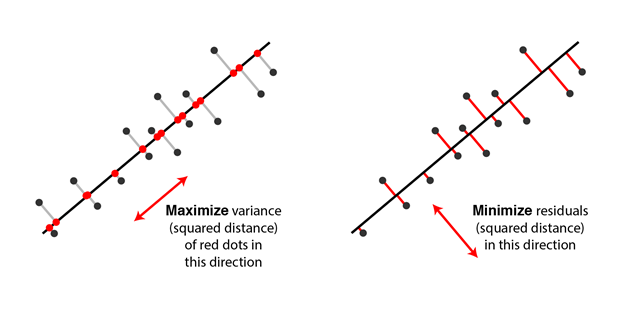
\includegraphics[width = 0.8\textwidth]{figures/pca_projection_explanation.png}
\label{pca_projection_explanation}
\end{figure}
Suppose we want to extract the first $k$ principal axis.
$$\mat{\hat{V}}_k = \argmin_{\mat{V}_k} \sum_{i=1}^{n} \norm{x_i - \mat{V}_k \mat{V}_k^Tx_i}^2 + \lambda \sum_{j=1}^{k}\norm{\beta_j}^2$$
$$\text{subject to }\mat{V}_k^T\mat{V}_k = \mat{I}_{k \times k}$$
where $x_i$ is the $i$th row of $\mat X$
\end{frame}
\subsection{Theorems}

\begin{frame}
\frametitle{Theorems}
Succes of PCA is due to the following two important optimal properties
\begin{enumerate}
\item Principal Components sequentially capture the maximum variability (among the columns of X, thus guaranteeing minimal information loss)
\item Principal Components are uncorrelated, (so we can talk about one principal component without referring to others)
\end{enumerate}
\end{frame}

\begin{frame}
\begin{thm}[Eckart-Young-Mirsky-Theorem]
Let $\widehat{\mat{A}}^* = \mat{U}_1 \mat{D}_1 \mat{V}_1^{\top}$
be the \textit{truncated singular value decomposition}. Then $\widehat{ \mat{A}}^*$ solves the matrix rank approximation problem

$$\min_{\operatorname{rank}(\widehat{\mat{A}}) \leq r} \|\mat{A}-\widehat{\mat{A}}\|_{\text{F}} = \|\mat{A}-\widehat{\mat{A}}^*\|_{\text{F}} = \sqrt{\sigma^2_{r+1} + \cdots + \sigma^2_m}$$

where $\sigma_i$ are the singular values of $\mat A$.
\end{thm}
\end{frame}

\begin{frame}
\begin{thm}
PCA is inconsistent for $p \gg n$.
\end{thm}
\end{frame}




\subsection{Limits of Usability}
\begin{frame}
\frametitle{Limits of Usability}
\begin{itemize}
\item Linear Relationship between variables
\item Correlation of variables
\item Completeness of data set
\item Outliers
\item Inconsistency theorem in $p \gg n$ case
\item Interpreation of principal axis
\end{itemize}


\end{frame}


\subsection{Application}
\begin{frame}
\frametitle{Application to handwritten digits}
\begin{figure}
\centering
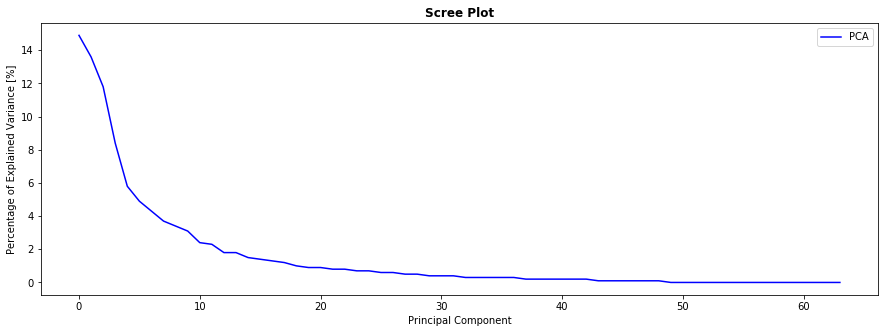
\includegraphics[width = 0.9\textwidth]{figures/pca_handwritten_digits_scree.png}
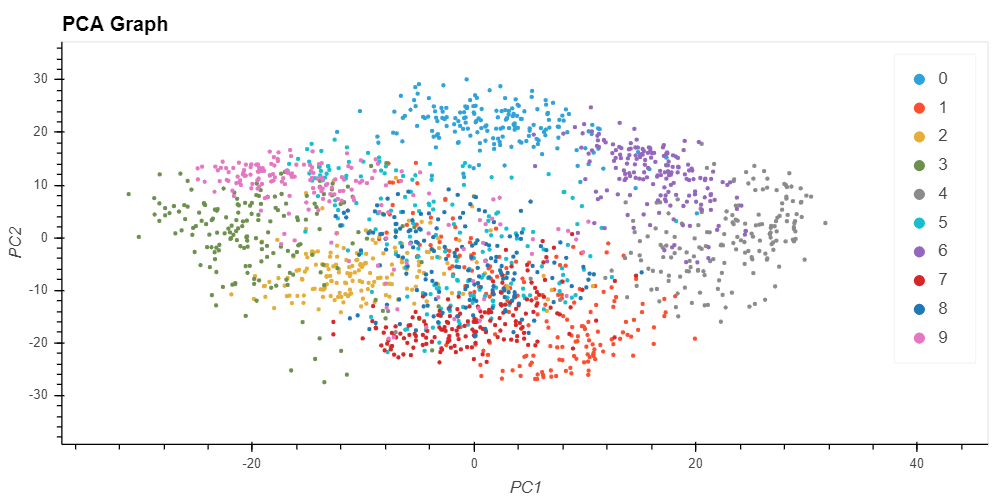
\includegraphics[width = 0.9\textwidth]{figures/pca_handwritten_digits.png}
\end{figure}
\end{frame}

%----------------------------------------------------------------------------------------
%	Fundamentals
%----------------------------------------------------------------------------------------

\section{Fundamentals}

\subsection{Regression}
\begin{frame}
\frametitle{Linear Regression}
Consider a linear regression model with $n$ observations and $p$ predictors. Let $Y = (y_1, \ldots , y_n)^T$ be the response vector and $\mat X = \left[X_1 \vert \cdots \vert X_p \right]$. We assume that all the $X_j$ and $Y$ are centered.

The linear regression model has the form
$$f(\mat X) = \beta_0 + \sum_{j=1}^p X_j\beta_j$$
where the $\beta_j$'s are unknown coefficients.

We define the residual sum of squares
$$RSS(\beta) = \sum_{i=1}^n (y_i - f(x_i))^2 = \sum_{i=1}^n (y_i - \beta_0 - \sum_{j=1}^p x_{ij}\beta_j)^2 = \norm{Y - \mat{X}\beta}_{2}^{2}$$

$$\hat{\beta} = \argmin_{\beta} RSS(\beta)$$
\end{frame}

\begin{frame}
\frametitle{Ridge Regression}
$$\hat{\beta}^{lasso} = \argmin_{\beta} \norm{Y - \mat{X}\beta}_{2}^{2} + \lambda \norm{\beta}_{2}^{2} = \sum_{i=1}^n (y_i - \beta_0 - \sum_{j=1}^p x_{ij}\beta_j)^2$$
$$\text{subject to } \norm{\beta}_{2}^2 \leq t$$
or equivalently in Lagrangian Form
$$\hat{\beta}^{lasso} = \argmin_{\beta}\left\{\frac{1}{2}\sum_{i=1}^n (y_i - \beta_0 - \sum_{j=1}^p x_{ij}\beta_j)^2 + \lambda\norm{\beta}_{2}^2 \right\}$$
\end{frame}

\begin{frame}
\frametitle{LASSO Regression}
\end{frame}

\begin{frame}
\frametitle{Elastic Net}
\end{frame}

\subsection{Sparsity inducing Norms}

%----------------------------------------------------------------------------------------
%	Sparse Principal Component Analysis
%----------------------------------------------------------------------------------------

\section{Sparse PCA}

\begin{frame}
\frametitle{Sparse PCA}
\textbf{Problem:} Principal Components are hard to interpret \linebreak
\textbf{Approach:} Require sparse loadings when performing PCA

$$\max{v^T \Sigma v}$$
$$\text{subject to } \norm{v}_2 = 1, \quad \norm{v}_{0} \leq k$$

\textbf{Relaxation}:
\begin{itemize}
\item a regression framework
\item a convex semidefinite programming framework
\item a generalized power method framework
\item an alternating maximization framework
\item forward-backward greedy search and exact methods using branch-and-bound techniques
\item Bayesian formulation framework
\end{itemize}
\end{frame}

\subsection{Mathematical Formulation}
\begin{frame}
\frametitle{Mathematical Formulation}
We will use a regression framework to derive sparse PCA. We add
$$(\hat{\mat{A}}, \hat{\mat{B}}) = \argmin_{\mat{A}, \mat{B}} \sum_{i=1}^{n} \norm{x_i - \mat{A}\mat{B}^Tx_i}^2 + \lambda \sum_{j=1}^{k}\norm{\beta_j}^2 + \sum_{j=1}^k \lambda_{1,j} \norm{\beta_j}_1$$
$$\text{subject to } \mat{A}^T\mat{A} = I_{k \times k}$$
\end{frame}

\subsection{Numerical Solution}

\begin{frame}
\begin{algorithm}[H]
  \scriptsize
    \caption{General SPCA Algorithm}
    \begin{algorithmic}[1]
        \Procedure{SPCA}{$A,B$}
        	\State $\mat A \gets \mat V[,1 \colon k]$, the loadings of the first k ordinary principal components
            \While{not converged} \Comment{Definiere Abbruchkriterium}
                \State Given a fixed $\mat A = [\alpha_1, \ldots, \alpha_k]$, solve the elastic net problem $$\beta_j = \argmin_{\beta} \norm{\mat X \alpha_j - \mat X \beta}^{2} + \lambda \norm{\beta}^2 + \lambda_{1,j}\norm{\beta}_{1}$$
                \State For a fixed $\mat B = [\beta_1, \ldots, \beta_k]$, compute the SVD of $$\mat X^T \mat X \mat B = \mat U \mat D \mat V^T$$
                \State $\mat A \gets \mat U \mat V^T$
            \EndWhile
            \State $\hat{V}_j = \frac{\beta_j}{\norm{\beta_j}}$ for $j = 1, \ldots, k$
        \EndProcedure
    \end{algorithmic}
\end{algorithm} 
\end{frame}

\subsection{Adjusted Variances}
\subsection{p >> n case}

%----------------------------------------------------------------------------------------
%	Application
%----------------------------------------------------------------------------------------

\section{Application}

\subsection{Dataset}
\subsection{Results}

%----------------------------------------------------------------------------------------
%	References
%----------------------------------------------------------------------------------------

\section{References}
\begin{frame}

\frametitle{References}

\begin{thebibliography}{9}
\bibitem[Beamerpaket]{paket} \emph{Beamer Paket} \\ 
\text{http://latex-beamer.sourceforge.net/}
\bibitem[Beamerdokumentation]{doku} \emph{User's Guide to the Beamer} 
\bibitem[Dante]{dante} \emph{DANTE e.V.} \text{http://www.dante.de}   
\end{thebibliography}


\end{frame}


\section{Appendix}

\end{document}
